%%%%%%%%%%%%%%%%%%%%%%%%%%%%%%%%%%%%%%%%%
% Programming/Coding Assignment
% LaTeX Template
%
% This template has been downloaded from:
% http://www.latextemplates.com
%
% Original author:
% Ted Pavlic (http://www.tedpavlic.com)
%
% Note:
% The \lipsum[#] commands throughout this template generate dummy text
% to fill the template out. These commands should all be removed when 
% writing assignment content.
%
% This template uses a Perl script as an example snippet of code, most other
% languages are also usable. Configure them in the "CODE INCLUSION 
% CONFIGURATION" section.
%
%%%%%%%%%%%%%%%%%%%%%%%%%%%%%%%%%%%%%%%%%

%----------------------------------------------------------------------------------------
%	PACKAGES AND OTHER DOCUMENT CONFIGURATIONS
%----------------------------------------------------------------------------------------

\documentclass{article}

\usepackage{fancyhdr} % Required for custom headers
\usepackage{lastpage} % Required to determine the last page for the footer
\usepackage{extramarks} % Required for headers and footers
\usepackage[usenames,dvipsnames]{color} % Required for custom colors
\usepackage{graphicx} % Required to insert images
\usepackage{subcaption}
\usepackage{listings} % Required for insertion of code
\usepackage{courier} % Required for the courier font
\usepackage{amsmath}
\usepackage{framed}

% Margins
\topmargin=-0.45in
\evensidemargin=0in
\oddsidemargin=0in
\textwidth=6.5in
\textheight=9.0in
\headsep=0.25in

\linespread{1.1} % Line spacing

% Set up the header and footer
\pagestyle{fancy}
\lhead{\hmwkAuthorName} % Top left header
\chead{\hmwkClass\ (\hmwkClassTime): \hmwkTitle} % Top center head
%\rhead{\firstxmark} % Top right header
\lfoot{\lastxmark} % Bottom left footer
\cfoot{} % Bottom center footer
\rfoot{Page\ \thepage\ of\ \protect\pageref{LastPage}} % Bottom right footer
\renewcommand\headrulewidth{0.4pt} % Size of the header rule
\renewcommand\footrulewidth{0.4pt} % Size of the footer rule

\setlength\parindent{0pt} % Removes all indentation from paragraphs

%----------------------------------------------------------------------------------------
%	CODE INCLUSION CONFIGURATION
%----------------------------------------------------------------------------------------

\definecolor{mygreen}{rgb}{0,0.6,0}
\definecolor{mygray}{rgb}{0.5,0.5,0.5}
\definecolor{mymauve}{rgb}{0.58,0,0.82}

\lstset{ %
  backgroundcolor=\color{white},   % choose the background color
  basicstyle=\footnotesize,        % size of fonts used for the code
  breaklines=true,                 % automatic line breaking only at whitespace
  captionpos=b,                    % sets the caption-position to bottom
  commentstyle=\color{mygreen},    % comment style
  escapeinside={\%*}{*)},          % if you want to add LaTeX within your code
  keywordstyle=\color{blue},       % keyword style
  stringstyle=\color{mymauve},     % string literal style
}

%----------------------------------------------------------------------------------------
%	DOCUMENT STRUCTURE COMMANDS
%	Skip this unless you know what you're doing
%----------------------------------------------------------------------------------------

% Header and footer for when a page split occurs within a problem environment
\newcommand{\enterProblemHeader}[1]{
%\nobreak\extramarks{#1}{#1 continued on next page\ldots}\nobreak
%\nobreak\extramarks{#1 (continued)}{#1 continued on next page\ldots}\nobreak
}

% Header and footer for when a page split occurs between problem environments
\newcommand{\exitProblemHeader}[1]{
%\nobreak\extramarks{#1 (continued)}{#1 continued on next page\ldots}\nobreak
%\nobreak\extramarks{#1}{}\nobreak
}

\setcounter{secnumdepth}{0} % Removes default section numbers
\newcounter{homeworkProblemCounter} % Creates a counter to keep track of the number of problems
\setcounter{homeworkProblemCounter}{0}

\newcommand{\homeworkProblemName}{}
\newenvironment{homeworkProblem}[1][Problem \arabic{homeworkProblemCounter}]{ % Makes a new environment called homeworkProblem which takes 1 argument (custom name) but the default is "Problem #"
\stepcounter{homeworkProblemCounter} % Increase counter for number of problems
\renewcommand{\homeworkProblemName}{#1} % Assign \homeworkProblemName the name of the problem
\section{\homeworkProblemName} % Make a section in the document with the custom problem count
\enterProblemHeader{\homeworkProblemName} % Header and footer within the environment
}{
\exitProblemHeader{\homeworkProblemName} % Header and footer after the environment
}

\newcommand{\problemAnswer}[1]{ % Defines the problem answer command with the content as the only argument
\noindent\framebox[\columnwidth][c]{\begin{minipage}{0.98\columnwidth}#1\end{minipage}} % Makes the box around the problem answer and puts the content inside
}

\newcommand{\homeworkSectionName}{}
\newenvironment{homeworkSection}[1]{ % New environment for sections within homework problems, takes 1 argument - the name of the section
\renewcommand{\homeworkSectionName}{#1} % Assign \homeworkSectionName to the name of the section from the environment argument
\subsection{\homeworkSectionName} % Make a subsection with the custom name of the subsection
\enterProblemHeader{\homeworkProblemName\ [\homeworkSectionName]} % Header and footer within the environment
}{
\enterProblemHeader{\homeworkProblemName} % Header and footer after the environment
}

%----------------------------------------------------------------------------------------
%	NAME AND CLASS SECTION
%----------------------------------------------------------------------------------------

\newcommand{\hmwkTitle}{Assignment 3} % Assignment title
\newcommand{\hmwkDueDate}{Friday, Mar. 19, 2018} % Due date
\newcommand{\hmwkClass}{CSC411} % Course/class
\newcommand{\hmwkClassTime}{LEC 5101/0101} % Class/lecture time
\newcommand{\hmwkAuthorName}{Zhongtian Ouyang/Yihao Ni} % Your name

%----------------------------------------------------------------------------------------
%	TITLE PAGE
%----------------------------------------------------------------------------------------

\title{
\vspace{2in}
\textmd{\textbf{\hmwkClass:\ \hmwkTitle}}\\
\normalsize\vspace{0.1in}\small{Due\ on\ \hmwkDueDate}\\
\vspace{0.1in}
\vspace{3in}
}

\author{\textbf{\hmwkAuthorName}}
\date{} % Insert date here if you want it to appear below your name

%----------------------------------------------------------------------------------------

\begin{document}

\maketitle
\clearpage
%----------------------------------------------------------------------------------------
%	PROBLEM 1
%----------------------------------------------------------------------------------------

% To have just one problem per page, simply put a \clearpage after each problem

\begin{homeworkProblem}
\noindent \textit{Useful keywords}\\
This dataset contains headlines with the word "trump", there are 1968 real news and 1268 fake news, with 4814 different words in those headlines. 

We choose "korea", "black" and "ban" to predict whether a news is real or fake. The following output is obtained by running part1() in fake.py.
\begin{framed}
Word "korea" appears 4.522\% in real news and 0.000\% in fake news.\\
Word "black" appears 0.051\% in real news and 3.236\% in fake news.\\
Word "ban" appears 5.335\% in real news and 1.464\% in fake news.
\end{framed}

From the output we can say that a news containing "korea" and "ban" is more likely to be a real news, while a news containing "black" is more likely to be a fake news.

\end{homeworkProblem}
\clearpage
%----------------------------------------------------------------------------------------
%	PROBLEM 2
%----------------------------------------------------------------------------------------

\begin{homeworkProblem}
\noindent \textit{Naive Bayes}\\
The best value for m, p is:(1, 0.4)\\
Performance on training set is 95.92\%\\
Performance on test set is 86.12\%\\
Performance on validation set is 87.16\%\\
To find the value for m and p, I trained the naive bayes with p = [0.1,0.2,...,1.0] and m = [1,2,3] using a for loop in the tune\_p2() function. And then choose the m, p that have the best result on the validation set as our optimal m, p value. \\
I use the formula in the following function when calculating probability to avoid underflow problem, because the probability could be very small. The function take in a list of small numbers and return their product.
\begin{framed}
\begin{lstlisting}[language=python]
def multi(nums):
    result = math.exp(sum(map(lambda x: math.log(x), nums)))
    return result
\end{lstlisting}
\end{framed}
\end{homeworkProblem}
\clearpage

%----------------------------------------------------------------------------------------
%	PROBLEM 3
%----------------------------------------------------------------------------------------

\begin{homeworkProblem}
\noindent \textit{More Naive Bayes}\\
Part 3b)\\
The words that we want are displayed below.\\
The formulas used for finding the words are folloiwng(m, p are 1 and 0.4):\\
(label is either fake or real, word is a single word, the words we want are the ones that have highest corresponding Probability)
\\
$p(label\mid word) = \frac{P(word\mid label)P(label)}{P(word)} = \frac{P(word	\ \cap \ label)}{P(word)} $\\
\\
$P(real\mid word\ exist) = \frac{P(word\ exist\ \cap\ real)}{P(word\ exist)} = \frac{count(headlines\ in\ training\ set\ that\ contain\ the\ word\ and\ is\ real) + mp}{count(headlines\ in\ training\ set\ that\ contain\ the\ word) + p}$\\
\\
$P(fake\mid word\ exist) = \frac{P(word\ exist\ \cap\ fake)}{P(word\ exist)} = \frac{count(headlines\ in\ training\ set\ that\ contain\ the\ word\ and\ is\ fake) + mp}{count(headlines\ in\ training\ set\ that\ contain\ the\ word) + p}$\\
\\
$P(real\mid word\ absent) = \frac{P(word\ absent\ \cap\ real)}{P(word\ absent)} = \frac{count(headlines\ in\ training\ set\ that\ not\ contain\ the\ word\ and\ is\ real) + mp}{count(headlines\ in\ training\ set\ that\ not\ contain\ the\ word) + p}$\\
\\
$P(fake\mid word\ absent) = \frac{P(word\ exist\ \cap\ fake)}{P(word\ exist)} = \frac{count(headlines\ in\ training\ set\ that\ not\ contain\ the\ word\ and\ is\ fake) + mp}{count(headlines\ in\ training\ set\ that\ not\ contain\ the\ word) + p}$\\

\begin{framed}
\begin{lstlisting}[language=python]
========================== Part 3a ==========================
10 words whose presence most strongly predicts that the news is real
['korea', 'turnbull', 'travel', 'trumps', 'australia', 'north', 'comments', 'ban', 'refugee', 'paris']
10 words whose absence most strongly predicts that the news is real
['trump', 'the', 'to', 'hillary', 'a', 'is', 'of', 'and', 'in', 'clinton']
10 words whose presence most strongly predicts that the news is fake
['black', 'breaking', 'u', 'woman', '3', 'soros', 'm', 'd', 'every', 'voter']
10 words whose absence most strongly predicts that the news is fake
['donald', 'trumps', 'us', 'says', 'korea', 'north', 'ban', 'turnbull', 'travel', 'wall']
\end{lstlisting}
\end{framed}
The absence of words influent more on predicting whether the headline is real or fake news. Even though P(label|word) is usually greater than P(label|not word). There are much more words that are absent than there are that are present. In a headline, at most 20 words are present, while about 4000 words are absent. So the absences contributes more on the final probability.\\
\clearpage
Part 3b)
\begin{framed}
\begin{lstlisting}[language=python]
========================== Part 3b ==========================
10 words whose presence most strongly predicts that the news is real
['korea', 'turnbull', 'travel', 'trumps', 'australia', 'north', 'comments', 'ban', 'refugee', 'paris']
10 words whose absence most strongly predicts that the news is real
['trump', 'hillary', 'clinton', 'just', 'new', 'win', 'america', 'obama', 'black', 'victory']
10 words whose presence most strongly predicts that the news is fake
['black', 'breaking', 'u', 'woman', '3', 'soros', 'm', 'd', 'voter', 'watch']
10 words whose absence most strongly predicts that the news is fake
['donald', 'trumps', 'says', 'korea', 'north', 'ban', 'turnbull', 'travel', 'wall', 'australia']
\end{lstlisting}
\end{framed}
Part3(c)\\
It might make sense to remove the stop words when interpreting the model because many of those stop words does not have real meaning. It's presence or absence should not influence our predictions on whether a headline is a fake one or a real one. But on the other hand, it might also helpful to keep the stopwords because some stop words may define the tune of the headline. And the fake or real news could have a preference in tune.
\end{homeworkProblem}
\clearpage
%----------------------------------------------------------------------------------------
%	PROBLEM 4
%----------------------------------------------------------------------------------------

\begin{homeworkProblem}
\noindent \textit{Training a logistic regression model}\\

We train the logistic regression model by pytorch using a linear model and a cross entropy loss. Weight\_decay in optimizer is chosen to be $5*10^{-3}$. The value is larger the better. But with a larger value than our choice, theta may not be trained to a suitable value, lowering the validation set performance.\\~\\
Following is the learning curves (performance vs. iteration) of the Logistic Regression model. 

\begin{figure}[!ht]
\centering
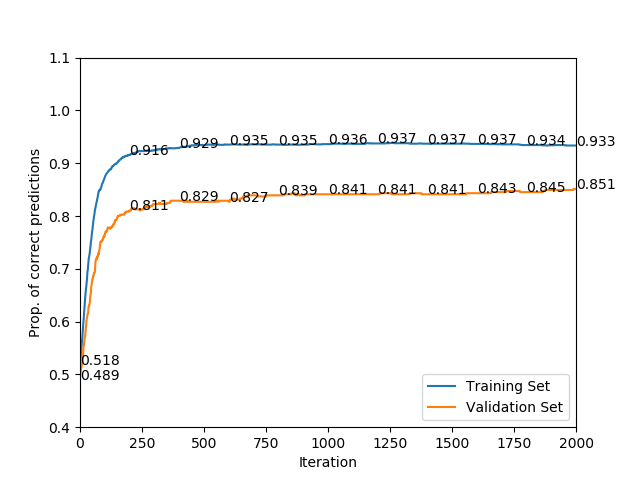
\includegraphics[width=1\linewidth]{p4.png}
\caption{performance}
\label{fig:p4w}
\end{figure}

The model performs fairly well after only several iterations, and the validation performance reaches its max at about 2000 iterations (tried more iterations but more iterations will lead to a poorer validation performance). The test performance under this model is as follows:
\begin{framed}
Test Set performance : 0.8326530612244898
\end{framed}

\end{homeworkProblem}
\clearpage

%----------------------------------------------------------------------------------------
%	PROBLEM 5
%----------------------------------------------------------------------------------------

\begin{homeworkProblem}
\noindent \textit{Formulation}\\
For logistic regression, $\theta_k$ is the weight of the kth keyword, if the weight is positive, then the a piece of news containing the kth keyword is more likely to be a real news, and vice versa. $I_k(x)$ is whether or not the kth keyword presents, 1 for presence and 0 for not. If the output is greater than a given threshold, we say the news is real, and if less than the threshold, we say the news is fake.

For naive bayes, the formula represent the log of the probability we calculated previously. $\theta_0$ is the bias, that is to say, it indicates the log probability of the news being real or fake given only the training set and there a headline that every word is absent. The formula for $\theta_0$ is the formula for $\beta_0$ on slide 26 of Genrative Classifiers PPT. In our case, y is the label, $X_1, X_2 .... = I_1(x), I_2(x) ....$. $\theta_j$ for $1 <= j <= k$ is the weight associated with the jth keyword. The formula for it is the formula for $\beta_j$ in the same slide. So when $I_j(x) = 0$, $\theta_j * I_j(x) = 0$, when $I_j(x) = 1$, the $-log\frac{p(x_j = 0\mid y = c)}{p(x_j = 0\mid y = c^\prime)}$ in  $\theta_j$ cancels out with $log\frac{p(x_j = 0\mid y = c)}{p(x_j = 0\mid y = c^\prime)}$ in $\theta_0$. So in the final formular only $log\frac{p(x_j = 1\mid y = c)}{p(x_j = 1\mid y = c^\prime)}$ is left. $I_j(x)$ is a function that return 1 if the jth keyword presents in the headline x,  and 0 for not. If the output for y=real is greater we say the news is real, and if output for y=fake is greater, we say the news is fake.
\end{homeworkProblem}
\clearpage
%----------------------------------------------------------------------------------------
%	PROBLEM 6
%----------------------------------------------------------------------------------------
\begin{homeworkProblem}
\noindent \textit{Words obtained using Logistic Regression}

For this problem, we get the value of theta by substracting the weight for the news to be fake from the weight for the news to be real given the presence of a keyword. This works as if the result is larger, the news is more likely to be real than fake, and vice versa.
\subsection{Part(a)}
\begin{framed}
\begin{lstlisting}[language=python]
========================== Part 6a ==========================
TOP 10 positive thetas with stop words: 
	1 : "ban"   with theta 0.2616
	2 : "scaramucci"   with theta 0.2545
	3 : "donald"   with theta 0.2479
	4 : "refugee"   with theta 0.2459
	5 : "us"   with theta 0.2443
	6 : "call"   with theta 0.2384
	7 : "climate"   with theta 0.2372
	8 : "trumps"   with theta 0.2367
	9 : "trade"   with theta 0.2367
	10 : "korea"   with theta 0.2351

TOP 10 negative thetas with stop words: 
	1 : "victory"   with theta -0.2762
	2 : "obama"   with theta -0.2566
	3 : "american"   with theta -0.2533
	4 : "they"   with theta -0.2533
	5 : "breaking"   with theta -0.2530
	6 : "hillary"   with theta -0.2522
	7 : "comment"   with theta -0.2498
	8 : "that"   with theta -0.2491
	9 : "america"   with theta -0.2481
	10 : "elect"   with theta -0.2460
\end{lstlisting}
\end{framed}

\subsection{Part(b)}
\begin{framed}
\begin{lstlisting}[language=python]
========================== Part 6b ==========================
TOP 10 positive thetas without stop words: 
	1 : "ban"   with theta 0.2616
	2 : "scaramucci"   with theta 0.2545
	3 : "donald"   with theta 0.2479
	4 : "refugee"   with theta 0.2459
	5 : "climate"   with theta 0.2372
	6 : "trumps"   with theta 0.2367
	7 : "trade"   with theta 0.2367
	8 : "korea"   with theta 0.2351
	9 : "debate"   with theta 0.2351
	10 : "business"   with theta 0.2343

TOP 10 negative thetas without stop words: 
	1 : "victory"   with theta -0.2762
	2 : "obama"   with theta -0.2566
	3 : "american"   with theta -0.2533
	4 : "breaking"   with theta -0.2530
	5 : "hillary"   with theta -0.2522
	6 : "comment"   with theta -0.2498
	7 : "america"   with theta -0.2481
	8 : "elect"   with theta -0.2460
	9 : "people"   with theta -0.2452
	10 : "black"   with theta -0.2438
\end{lstlisting}
\end{framed}

\subsection{Part(c)}
Using the magnitude of the logistic regression parameters to indicate the importance of a feature is a bad idea in general. The reason is that for features that are not normalized, points which are outliers may influence the model a lot which can lower the performance. But in this problem, values vary from 0 and 1, therefore using magnitude will not cause such accuracy problem.


\end{homeworkProblem}
\clearpage
%----------------------------------------------------------------------------------------
%	PROBLEM 7
%----------------------------------------------------------------------------------------
\begin{homeworkProblem}
\noindent \textit{Decision tree}\\
Part 7a)\\
Performance on training set is 96.45\%\\
Performance on validation set is 79.42\%\\
Performance on test set is 75.10\%\\
i have tried with depth [1,10,20,30,....,150]. I choose depth 90 as it return the best result on validation set with the current tree configuration.\\
Other settings changes:\\
1. I change splitter to random. As it can be used to prevent overfitting the training set by not strictly selecting the best split and it has better performance\\
2. I set min\_samples\_split to 10 so that some very detailed features of the training set is not captured by the model\\
3. I set max\_features to 0.1, so everytime the model just consider 10\% of all the features. Also preventing overfitting. I have also tried log2, sqrt, and various percentages, and 0.1 seems to perform best\\
4. Random\_state is set to 0 as a random seed.
\begin{figure}[!ht]
\centering
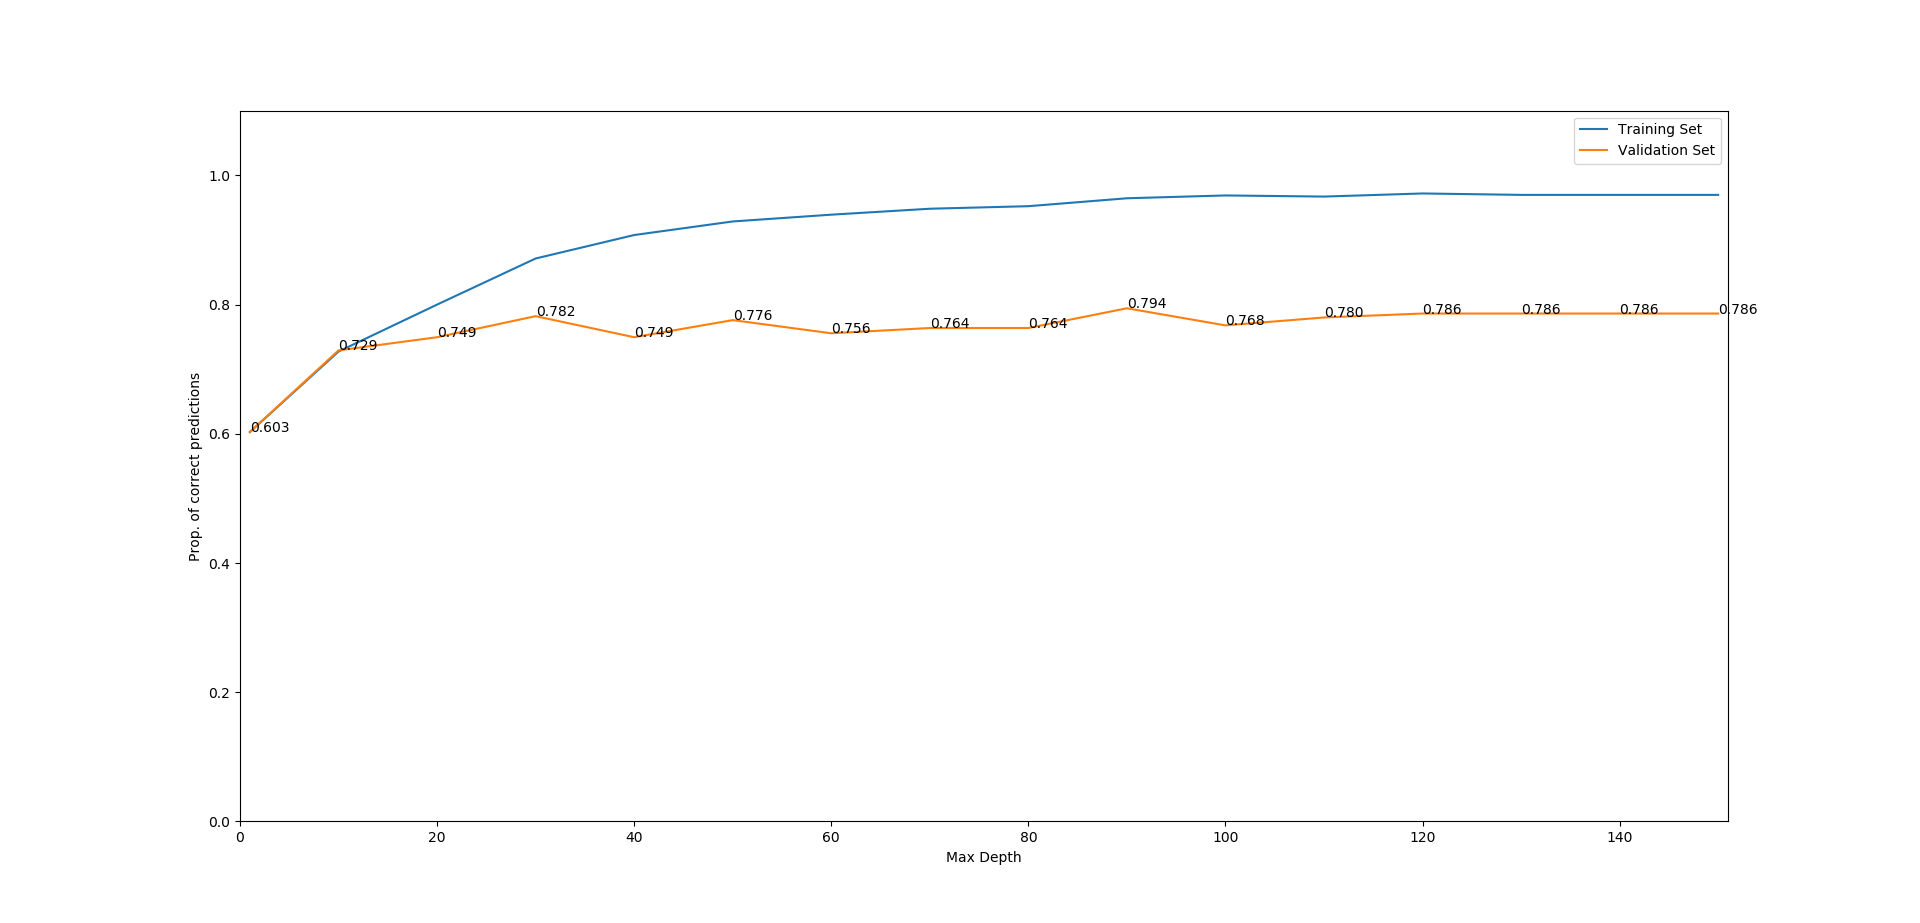
\includegraphics[width=1\linewidth]{p7.png}
\caption{Relation between max depth and performance}
\label{fig:p7}
\end{figure}
\clearpage
Part 7b)\\
The visualization is done using graphviz. The most important feature here is the word `korea', which is also the most important word whose presence most strongly predicts that the news is real in part 3, and one of the words correspond to the top 10 positive thetas in part 6. And the second important feature `black' can also be found in both part 3 and part 6 solution.\\
\begin{figure}[!ht]
\centering
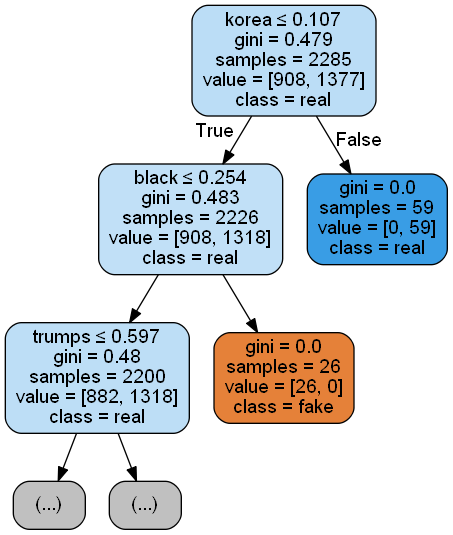
\includegraphics[width=0.4\linewidth]{DT.png}
\caption{Decision Tree}
\label{fig:p7}
\end{figure}
\\
Part 7c)\\
\begin{center}
\begin{tabular}{ |c|c|c|c| } 
 \hline
  						& Naive Bayes 	& Logistic Regression 	& Decision Tree \\ 
 Training Set		& 95.92\% 		& 93.34\% 				&96.45\%\\ 
 Validation Set 	& 87.16\%			& 85.13\%					&79.42\%\\ 
 Test Set 			& 86.12\% 		& 83.26\%					&75.10\%\\
 \hline
\end{tabular}
\end{center}
From the above Table, we can see that Naive Bayes perform the best which is as expected. Logictic Regression's performance is off by a bit. And Decision Tree perform the worst with only 75.10\% on test set. Decision Tree also overfit the most with a 17\% perforamance difference between training set and validation set.
\end{homeworkProblem}
\clearpage
%----------------------------------------------------------------------------------------
%	PROBLEM 8
%----------------------------------------------------------------------------------------
\begin{homeworkProblem}
\noindent \textit{Information Gain}\\
Part 8a)\\
The information gain of the split on the word `korea' is calculate with IY\_x(`Korea'). The result is 0.01919077990760476\\
\begin{framed}
\begin{lstlisting}[language=python]
def PL(num):
    if num != 0:
        return (-num) * math.log(num, 2)
    else:
        return 0  # to account for the case where num is 0
        
def IY_x(word):
    # H(Y) = Sum(-P(Y=y)logP(Y=y))for y=real,fake
    fake_count = len(Sets[TRAINING_FAKE])
    real_count = len(Sets[TRAINING_REAL])
    total_count = fake_count + real_count
    P_y_fake = fake_count / (fake_count + real_count)
    P_y_real = real_count / (fake_count + real_count)
    H_Y = PL(P_y_fake) + PL(P_y_real)
    # H(Y|xi) = P(xi=0)[-P(y=real|xi=0)logP(y=real|xi=0) + -P(y=fake|xi=0)logP(y=fake|xi=0)]+
    #           P(xi=1)[-P(y=real|xi=1)logP(y=real|xi=1) + -P(y=fake|xi=1)logP(y=fake|xi=1)]
    xi_count = Count[word][FAKE] + Count[word][REAL]
    p_xi_1 = xi_count / total_count
    p_xi_0 = 1 - p_xi_1
    p_y_fake_xi_1 = Count[word][FAKE] / xi_count
    p_y_real_xi_1 = Count[word][REAL] / xi_count
    if xi_count == total_count:
        p_y_fake_xi_0, p_y_real_xi_0 = 1, 1
    else:
        p_y_fake_xi_0 = (fake_count - Count[word][FAKE]) / (total_count - xi_count)
        p_y_real_xi_0 = (real_count - Count[word][REAL]) / (total_count - xi_count)
    H_Y_xi = p_xi_0 * (PL(p_y_real_xi_0) + PL(p_y_fake_xi_0)) + p_xi_1 * (PL(p_y_real_xi_1) + PL(p_y_fake_xi_1))

    return H_Y - H_Y_xi
\end{lstlisting}
\end{framed}
Part 8b)\\
The information gain of the split on the word `wall' is calculate with IY\_x(`wall'). The result is 0.0032532196874575092. This value is smaller than the previous value in part a) as expected since the word `korea', being the first split word shoud be one of the words with highest information gain.\\
 However, both values are pretty small. The reason is that in our training set, there are no words that appears a lot and almost only appears in either fake or real news, which would have a much higher information gain. \\
For example, If we have a word which appears everytime in the fake news, and never in the real news. Then the I(Y,test word) will be equal to H(Y) which is 0.969\\
\end{homeworkProblem}
\clearpage
%----------------------------------------------------------------------------------------

\end{document}
